\documentclass[a4paper]{article}
\usepackage{listings}
\usepackage[utf8]{inputenc}
\usepackage[utf8]{vietnam}
\usepackage[english]{babel}
\usepackage{a4wide,amssymb,epsfig,latexsym,multicol,array,hhline,fancyhdr}
\usepackage{amsmath}
\usepackage{lastpage}
\usepackage[lined,boxed,commentsnumbered]{algorithm2e}
\usepackage{enumerate}
\usepackage{color}
\usepackage{graphicx}		
\usepackage{tabularx, caption}
\usepackage{multirow}
\usepackage{multicol}
\usepackage{rotating}
\usepackage{graphics}
\usepackage{geometry}
\geometry{ a4paper,left=30mm, right=25mm, top=20mm, bottom=30mm}
\usepackage{setspace}
\usepackage{epsfig}
\usepackage{tikz}
\usepackage{ragged2e}
\usetikzlibrary{arrows,snakes,backgrounds}
\usepackage{hyperref}
\hypersetup{urlcolor=blue,linkcolor=black,citecolor=black,colorlinks=true} 
\usepackage{pstcol} 		

% Typesetting Listings
\usepackage{xcolor}
\usepackage{color}
\definecolor{listinggray}{gray}{0.9}
\definecolor{lbcolor}{rgb}{0.9,0.9,0.9}
\definecolor{Darkgreen}{rgb}{0.1,0.6,0.1}
\definecolor{whitesmoke}{rgb}{0.99, 0.99,0.99}

\lstset{
	backgroundcolor=\color{whitesmoke},
	tabsize=2,
	language=[GNU]C++,
	basicstyle=\scriptsize,
	upquote=true,
	aboveskip={1.5\baselineskip},
	columns=fixed,
	showstringspaces=false,
	extendedchars=false,
	breaklines=true,
	prebreak = \raisebox{0ex}[0ex][0ex]{\ensuremath{\hookleftarrow}},
	frame=single,
	numbers=left,
	showtabs=false,
	showspaces=false,
	showstringspaces=false,
	identifierstyle=\ttfamily,	
	keywordstyle=\color[rgb]{0,0,1},
	commentstyle=\color[rgb]{0.026,0.112,0.095},
	stringstyle=\color[rgb]{0.627,0.126,0.941},
	numberstyle=\color[rgb]{0.205, 0.142, 0.73},
	%\lstdefinestyle{C++}{language=C++,style=numbers}’.
}
\lstset{
	backgroundcolor=\color{whitesmoke},
	tabsize=2,
	language=C++,
	captionpos=b,
	frame=lines,
	numbers=left,
	numberstyle=\tiny,
	numbersep=5pt,
	breaklines=true,
	showstringspaces=false,
	basicstyle=\footnotesize,
	%identifierstyle=\color{magenta},
	keywordstyle=\color[rgb]{0,0,1},
	commentstyle=\color{Darkgreen},
	stringstyle=\color{red}
}				

% begin format Header and Footer
%\usepackage{fancyhdr}
\setlength{\headheight}{30pt}
\pagestyle{fancy}
\fancyhead{} % clear all header fields
\fancyhead[L]{
 \begin{tabular}{rl}
    \begin{picture}(25,15)(0,0)
    \put(0,-8){
\includegraphics[width=8mm, height=8mm]{images/LogoBK.png}}
    %\put(0,-8){\epsfig{width=10mm,figure=hcmut.eps}}
   \end{picture}&
	%\includegraphics[width=8mm, height=8mm]{hcmut.png} & %
	\begin{tabular}{l}
		\textbf{\bf \ttfamily Đại Học Quốc Gia Tp. Hồ Chí Minh - Đại Học Bách Khoa}\\
		\textbf{\bf \ttfamily Khoa Khoa Học - Kĩ Thuật Máy Tính}
	\end{tabular} 	
 \end{tabular}
}
\fancyhead[R]{
	\begin{tabular}{l}
		\tiny \bf \\
		\tiny \bf 
	\end{tabular}  }
\fancyfoot{} % clear all footer fields
\fancyfoot[L]{\scriptsize \ttfamily Report: Assignment 2 - Operating Systems - Semester 192}
\fancyfoot[R]{\scriptsize \ttfamily Page {\thepage}/\pageref{LastPage}}
\renewcommand{\headrulewidth}{0.3pt}
\renewcommand{\footrulewidth}{0.3pt}
% end format Header and Footer

%%%
\setcounter{secnumdepth}{4}
\setcounter{tocdepth}{2}
\makeatletter
\newcounter {subsubsubsection}[subsubsection]
\renewcommand\thesubsubsubsection{\thesubsubsection .\@alph\c@subsubsubsection}
\newcommand\subsubsubsection{\@startsection{subsubsubsection}{4}{\z@}%
                                     {-3.25ex\@plus -1ex \@minus -.2ex}%
                                     {1.5ex \@plus .2ex}%
                                     {\normalfont\normalsize\bfseries}}
\newcommand*\l@subsubsubsection{\@dottedtocline{3}{10.0em}{4.1em}}
\newcommand*{\subsubsubsectionmark}[1]{}
\makeatother

\begin{document} % begin document

\begin{titlepage} % begin title page
\begin{center}
ĐẠI HỌC QUỐC GIA THÀNH PHỐ HỒ CHÍ MINH \\
TRƯỜNG ĐẠI HỌC BÁCH KHOA \\
KHOA KHOA HỌC - KỸ THUẬT MÁY TÍNH 
\end{center}
\vspace{1cm}
\begin{figure}[h!]
\begin{center}

\includegraphics[width=4cm]{images/LogoBK.png}
\end{center}
\end{figure}
\vspace{1cm}
\begin{center}
\begin{tabular}{c}
\multicolumn{1}{c}{\textbf{{\Large Report: Assignment 2 - Operating System }}}\\
~~\\

\hline
\\
\multicolumn{1}{l}{\textbf{{\Large Topic}}}\\
\\
\textbf{{\Huge Simple Operating System}}\\
\\
\hline
\end{tabular}
\end{center}
\vspace{0.5cm}
\vspace{0.5cm}
\begin{table}[h]
\hspace{5cm} 
\begin{tabular}{ll}
    Lecturer: & Nguyễn Hoài Nam\\
    Group 3 & Students:\\
   		& Nguyễn Long Kim - 1812742 \\
		& Nguyễn Duy Kiên - 1812704 \\
		& Nguyễn Văn Khang - 1812554 \\
		& Nguyễn Anh Khoa - 1812649 \\
\end{tabular}
\end{table}
\vspace{5cm}
\begin{center}
{\footnotesize TP. HỒ CHÍ MINH, THÁNG 6/2020}
\end{center}
\end{titlepage} % end title page

\newpage
\textbf{Task assingment}
\begin{center}
    \begin{tabular}{|p{3cm}|p{7cm}|p{2.5cm}|p{3cm}|}
        \hline
         Members: & Task : & Due date: & Accomplished date:\\
         \hline
          Nguyễn Duy Kiên &
          \begin{itemize}
              	\item Implement functions: enqueue() and dequeue() in queue.c
		\item Draw Gantt chart for sched\_0
		\item Answer the question in section Scheduler
          \end{itemize} &
          24/6/20220 &
	23/6/2020 \\
         \hline
          Nguyễn Văn Khang &
          \begin{itemize}
              	\item Implement functions: get\_proc() in sched.c
              	\item Draw Gantt chart for sched\_1
		\item Answer the question in section Scheduler
          \end{itemize} &
          24/6/20220 &
	23/6/2020 \\
         \hline
          Nguyễn Anh Khoa &
          \begin{itemize}
              	\item Implement functions: translate() and get\_page\_table() in mem.c
             	\item Show status of RAM after each allocation and deallocation function call in m0
		\item Answer the question in section Memory Management
          \end{itemize} &
          24/6/20220 &
	23/6/2020 \\
         \hline
          Nguyễn Long Kim &
          \begin{itemize}
              	\item Implement functions: alloc\_mem() and free\_mem() in mem.c
              	\item Show status of RAM after each allocation and deallocation function call in m1	
		\item Synchronization for [\_ram] access in mem.c
		\item Write report
          \end{itemize} &
          24/6/20220 &
	23/6/2020 \\
        \hline
    \end{tabular}
\end{center}

% Table of contents
\newpage
\tableofcontents

\newpage
\section{Scheduler}
\subsection{Question \& Answer}
\textbf{Question}: What is the advantage of using priority feedback queue in comparison with other scheduling algorithms you have learned?\\
\textbf{Answer}:
\begin{itemize}
	\item Thời gian đợi trung bình giảm so với giải thuật First Come First Served
	\item CPU chạy các process theo Round-Robin "style" nên đảm bảo tính công về thời gian thực thi của các process. Không có process nào được chạy quá thời gian mà OS cho phép, từ đó dẫn đến tránh được tình trạng trì hoãn vô hạn định xảy ra ở một số giải thuật định thời khác như:  Priority scheduling hay Multilevel Queue Scheduling  
	\item Sử dụng hai hàng đợi  $ ready\_queue $ và $ run\_queue $, các process được chuyển qua lại giữa hai hàng đợi này đến khi các process được hoàn tất, tăng thời gian đáp ứng cho các process do các process có độ ưu tiên thấp đến sau vẫn có thể được thực thi trước các process có độ ưu tiên cao hơn (vì có thể lúc này process có độ ưu tiên cao hơn đang ở $ run\_queue $).
\end{itemize}
\subsection{Gantt chart}
\textbf{Requirement:} Draw Gantt diagram describing how processes are executed by the CPU
\subsubsection{Test sched\_0}
\begin{itemize}
	\item \textbf{sched\_0 log}
		\lstinputlisting{logs/sched_0.log}
	\item \textbf{Gantt chart}
		\begin{figure}[h!]
		    \centering
		    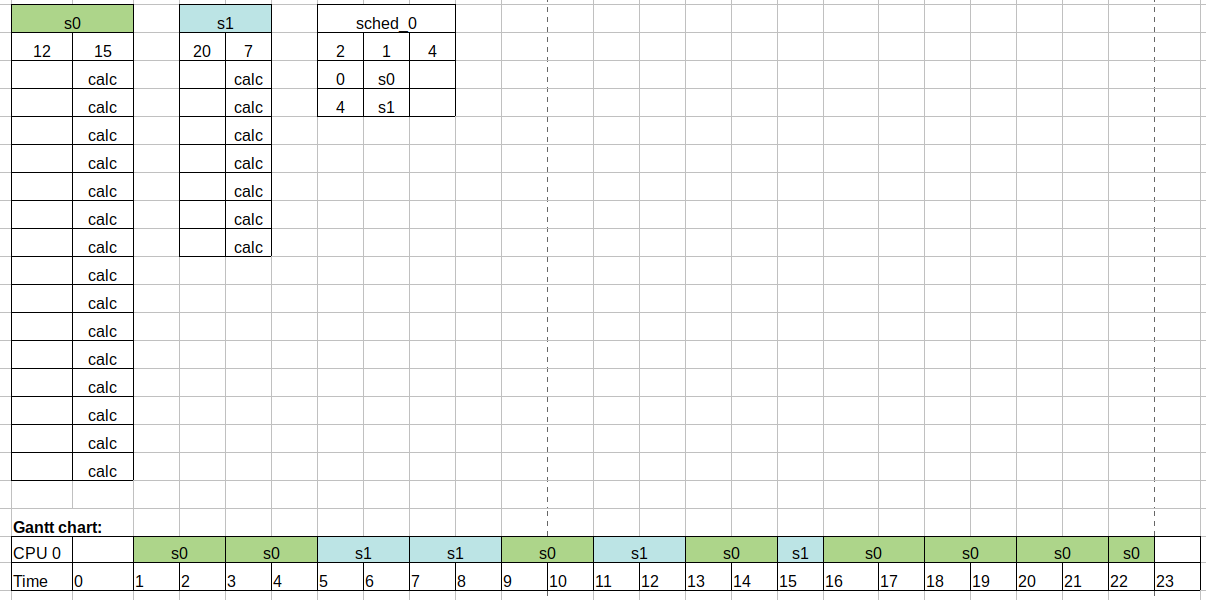
\includegraphics[width=16cm]{images/sched_0.png}
		    \caption{Gantt chart CPU thực thi các process trong sched\_0}
		    \label{fig:my_label}
		\end{figure}
\end{itemize}
\subsubsection{Test sched\_1}
\begin{itemize}
	\item \textbf{sched\_1 log}
		\lstinputlisting{logs/sched_1.log}
	\item \textbf{Gantt chart}
		\begin{figure}[h!]
		    \centering
		    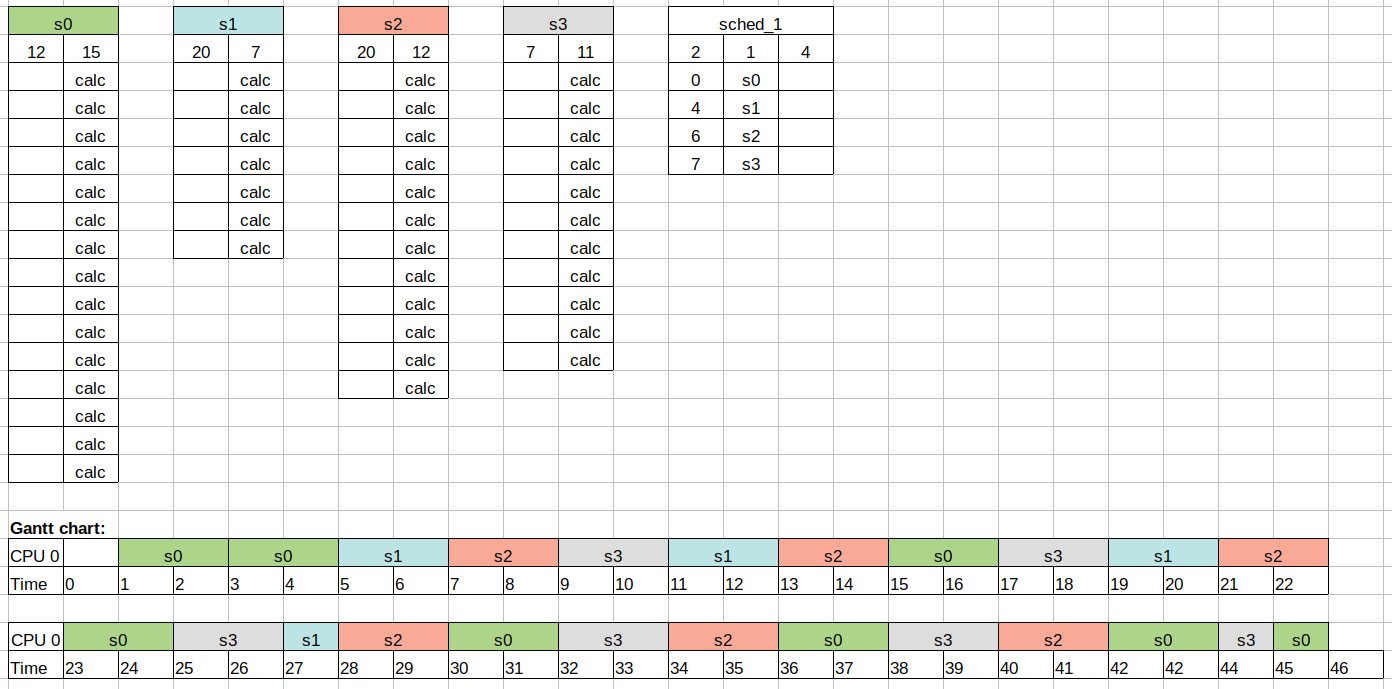
\includegraphics[width=16cm]{images/sched_1.png}
		    \caption{Gantt chart CPU thực thi các process trong sched\_1}
		    \label{fig:my_label}
		\end{figure}
\end{itemize}

\newpage
\section{Memory management}
\subsection{Question \& Answer}
\textbf{Question}: What is the advantage and disadvantage of segmentation with paging?\\
\textbf{Answer}:
\begin{itemize}
	\item \textbf{Advantage:}
		\begin{itemize}
			\item Tiết kiệm bộ nhớ, sử dụng bộ nhớ hiệu quả, khắc phục việc kích thước bảng phân trang quá lớn
			\item Khắc phục được phân mảnh ngoại
		\end{itemize}
	\item \textbf{Disadvantage:}
		\begin{itemize}
			\item Chưa khắc phục được hiện tượng phân mảnh nội
		\end{itemize}
\end{itemize}
\subsection{Show status of RAM}
\textbf{Requirement:} Show the status of RAM after each memory allocation and deallocation function call
\subsubsection{Test $ m0 $}
\begin{itemize}
	\item \textbf{Below is content of file $ m0 $}
		\lstinputlisting{input/m0}
	\item \textbf{Status of RAM after each allocation and deallocation function call in $ m0 $}
		\lstinputlisting{logs/mem0.log}
\end{itemize}
\subsubsection{Test $ m1 $}
\begin{itemize}
	\item \textbf{Below is content of file $ m1 $}
		\lstinputlisting{input/m1}
	\item \textbf{Status of RAM after each allocation and deallocation function call in $ m1 $}
		\lstinputlisting{logs/mem1.log}
\end{itemize}

\section{Put it all together}
\subsection{Synchronization}
Trong file  $ mem.c $, hai hàm $ read\_mem() $ và $ write\_mem() $ truy cập vào $ [\_ram] $ có thể xảy ra bất đồng bộ nên ta cần thêm một $ mutex\_lock $: $ ram\_lock $ để giải quyết, khi đó hai hàm trên được chỉnh lại như sau:
\begin{itemize}
	\item \textbf{Hàm read\_mem()}
		\lstinputlisting{code/read_mem.c}
	\item \textbf{Hàm write\_mem()}
		\lstinputlisting{code/write_mem.c}
\end{itemize}
\subsection{Result of simulation}
\begin{itemize}
	\item \textbf{os\_0 log}
		\lstinputlisting{logs/os_0.log}
	\item \textbf{os\_1 log}
		\lstinputlisting{logs/os_1.log}
\end{itemize}

\end{document}